\documentclass[border=16pt]{standalone}
\usepackage[T1]{fontenc}
\usepackage[utf8]{inputenc}
\usepackage{circuitikz}
\usepackage{amsmath,amssymb}
\usetikzlibrary{positioning,calc}
\ctikzset{bipoles/length=1.15cm, font=\small}

% FONDO BLANCO (imprimible)
\definecolor{tinta}{HTML}{1E293B}
\definecolor{ambar}{HTML}{C2410C}
\definecolor{azul}{HTML}{0E7490}
\definecolor{verde}{HTML}{15803D}
\definecolor{rojo}{HTML}{B91C1C}
\definecolor{gris}{HTML}{6B7280}
\definecolor{panel}{HTML}{F1F5F9}

\begin{document}
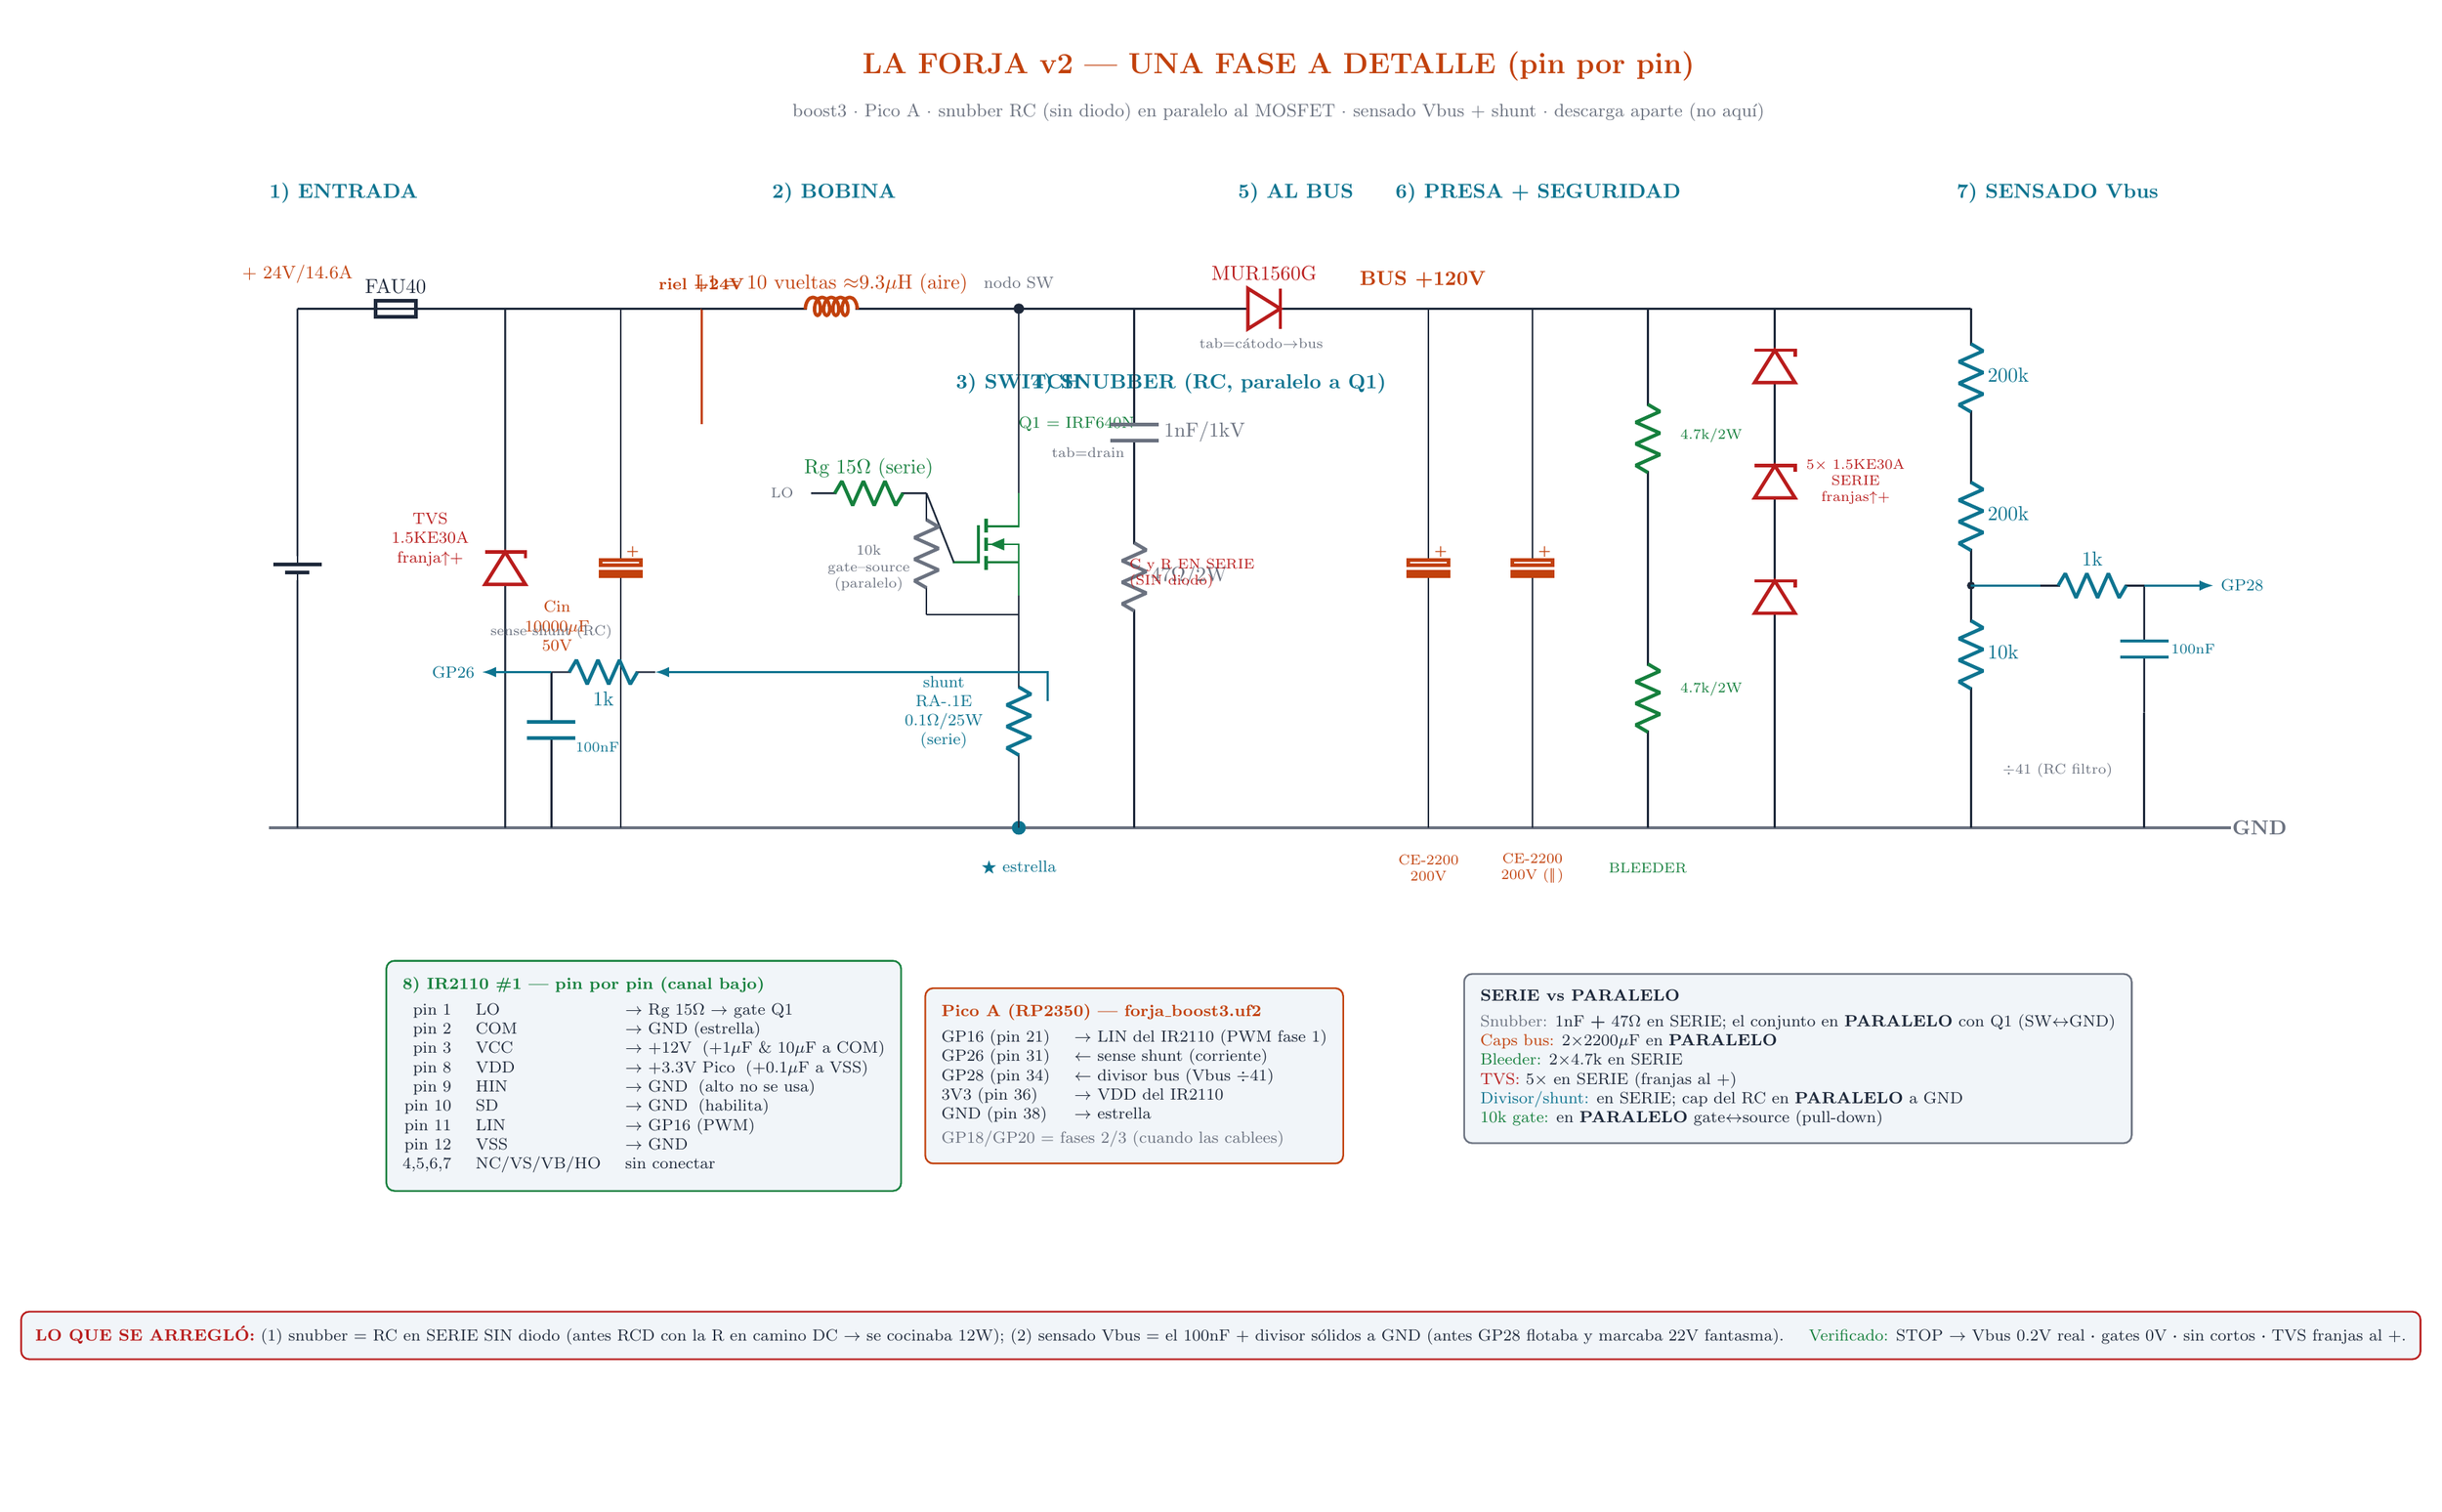
\begin{tikzpicture}[color=tinta, every node/.style={text=tinta}, line width=0.85pt]
\fill[white] (-6.5,-20.5) rectangle (30.5,5.0);

% ===================== TITULO =====================
\node[text=ambar, font=\bfseries\Large] at (12,4.2) {LA FORJA v2 — UNA FASE A DETALLE (pin por pin)};
\node[text=gris, font=\small] at (12,3.4) {boost3 · Pico A · snubber RC (sin diodo) en paralelo al MOSFET · sensado Vbus + shunt · descarga aparte (no aquí)};

% ===================== RIEL GND =====================
\draw[gris, line width=1.2pt] (-5.5,-9) -- (28.5,-9);
\node[text=gris, font=\bfseries] at (29,-9){GND};
\fill[azul] (7.5,-9) circle (0.12);
\node[text=azul, font=\footnotesize, align=center] at (7.5,-9.7){$\bigstar$ estrella};

% ===================== 1) ENTRADA =====================
\node[text=azul, font=\bfseries] at (-4.2,2.0){1) ENTRADA};
\draw (-5.0,0) to[battery1] (-5.0,-9);
\node[text=ambar, font=\small, align=center] at (-5.0,0.6){+ 24V/14.6A};
\draw (-5.0,0) -- (-4.2,0);
\draw (-4.2,0) to[fuse, l=\textcolor{tinta}{FAU40}] (-2.4,0);
\draw (-2.4,0) -- (2.0,0);
\draw (-1.4,0) to[empty Zener diode, invert, color=rojo] (-1.4,-9);
\node[text=rojo, font=\footnotesize, align=center] at (-2.7,-4.0){TVS\\1.5KE30A\\franja$\uparrow$+};
\draw (0.6,0) to[ecapacitor, color=ambar] (0.6,-9);
\node[text=ambar, font=\footnotesize, align=center] at (-0.5,-5.5){Cin\\10000$\mu$F\\50V};
\draw[ambar, line width=1.1pt] (2.0,0) -- (2.0,-2);
\node[text=ambar, font=\bfseries\footnotesize] at (2.0,0.4){riel +24V};

% ===================== 2) BOBINA =====================
\node[text=azul, font=\bfseries] at (4.3,2.0){2) BOBINA};
\draw (2.0,0) to[L, l=\textcolor{ambar}{L1 = 10 vueltas $\approx$9.3$\mu$H (aire)}, color=ambar] (6.5,0);
\draw (6.5,0) -- (9.5,0) coordinate(SW);
\fill[tinta] (7.5,0) circle (0.09);
\node[font=\footnotesize, text=gris] at (7.5,0.45){nodo SW};

% ===================== 3) MOSFET (switch) =====================
\node[text=azul, font=\bfseries] at (7.5,-1.3){3) SWITCH};
\node[nigfete, anchor=D, color=verde, scale=1.15] (Q) at (7.5,-3.2){};
\draw (SW) -- (7.5,0) -- (Q.D);
\node[text=verde, font=\footnotesize, align=left] at (8.5,-2.0){Q1 = IRF640N};
\node[text=gris, font=\scriptsize, align=left] at (8.7,-2.5){tab=drain};
% gate: Rg en serie + 10k gate-source en paralelo
\draw (Q.G) -- (5.9,-3.2);
\draw (5.9,-3.2) to[R, l_=\textcolor{verde}{Rg 15$\Omega$ (serie)}, color=verde] (3.9,-3.2);
\node[font=\scriptsize, text=gris] at (3.4,-3.2){LO};
\draw (5.9,-3.2) to[R, color=gris] (5.9,-5.3);
\node[text=gris, font=\scriptsize, align=center] at (4.9,-4.5){10k\\gate--source\\(paralelo)};
\draw (5.9,-5.3) -- (7.5,-5.3);     % al source (no a GND): pull-down gate-source
% source -> shunt -> GND
\draw (Q.S) -- (7.5,-5.3);
\draw (7.5,-5.3) to[R, color=azul] (7.5,-9);
\node[text=azul, font=\footnotesize, align=center] at (6.2,-7.0){shunt\\RA-.1E\\0.1$\Omega$/25W\\(serie)};

% ===================== 4) SNUBBER RC (paralelo al MOSFET) =====================
\node[text=azul, font=\bfseries] at (10.8,-1.3){4) SNUBBER (RC, paralelo a Q1)};
\draw (9.5,0) -- (9.5,-1.0);
\draw (9.5,-1.0) to[C, l=\textcolor{gris}{1nF/1kV}, color=gris] (9.5,-3.3);
\draw (9.5,-3.3) to[R, l=\textcolor{gris}{47$\Omega$/2W}, color=gris] (9.5,-6.0);
\draw (9.5,-6.0) -- (9.5,-9);
\node[text=rojo, font=\scriptsize, align=left] at (10.5,-4.6){C y R EN SERIE\\(SIN diodo)};

% ===================== 5) DIODO AL BUS =====================
\node[text=azul, font=\bfseries] at (12.3,2.0){5) AL BUS};
\draw (9.5,0) -- (10.5,0);
\draw (10.5,0) to[D, l=\textcolor{rojo}{MUR1560G}, color=rojo] (13.0,0);
\node[text=gris, font=\scriptsize] at (11.7,-0.6){tab=cátodo$\to$bus};
\draw (13.0,0) -- (24.0,0);
\node[text=ambar, font=\bfseries] at (14.5,0.5){BUS +120V};

% ===================== 6) BUS: caps ‖ bleeder ‖ TVS =====================
\node[text=azul, font=\bfseries] at (16.5,2.0){6) PRESA + SEGURIDAD};
\draw (14.6,0) to[ecapacitor, color=ambar] (14.6,-9);
\node[text=ambar, font=\scriptsize, align=center] at (14.6,-9.7){CE-2200\\200V};
\draw (16.4,0) to[ecapacitor, color=ambar] (16.4,-9);
\node[text=ambar, font=\scriptsize, align=center] at (16.4,-9.7){CE-2200\\200V (‖)};
\draw (18.4,0) to[R, color=verde] (18.4,-4.5);
\draw (18.4,-4.5) to[R, color=verde] (18.4,-9);
\node[text=verde, font=\scriptsize, align=center] at (19.5,-2.2){4.7k/2W};
\node[text=verde, font=\scriptsize, align=center] at (19.5,-6.6){4.7k/2W};
\node[text=verde, font=\scriptsize] at (18.4,-9.7){BLEEDER};
\draw (20.6,0) to[empty Zener diode, invert, color=rojo] (20.6,-2.0);
\draw (20.6,-2.0) to[empty Zener diode, invert, color=rojo] (20.6,-4.0);
\draw (20.6,-4.0) to[empty Zener diode, invert, color=rojo] (20.6,-6.0);
\draw (20.6,-6.0) -- (20.6,-9);
\node[text=rojo, font=\scriptsize, align=center] at (22.0,-3.0){5$\times$ 1.5KE30A\\SERIE\\franjas$\uparrow$+};

% ===================== 7) SENSADO Vbus =====================
\node[text=azul, font=\bfseries] at (25.5,2.0){7) SENSADO Vbus};
\draw (24.0,0) to[R, l=\textcolor{azul}{200k}, color=azul] (24.0,-2.4);
\draw (24.0,-2.4) to[R, l=\textcolor{azul}{200k}, color=azul] (24.0,-4.8);
\draw (24.0,-4.8) to[R, l=\textcolor{azul}{10k}, color=azul] (24.0,-7.2);
\draw (24.0,-7.2) -- (24.0,-9);
\fill[tinta] (24.0,-4.8) circle (0.07);
\draw[azul] (24.0,-4.8) -- (25.2,-4.8);
\draw (25.2,-4.8) to[R, l=\textcolor{azul}{1k}, color=azul] (27.0,-4.8);
\draw (27.0,-4.8) to[C, color=azul] (27.0,-7.0);
\node[text=azul, font=\scriptsize] at (27.85,-5.9){100nF};
\draw (27.0,-7.0) -- (27.0,-9);
\draw[azul,-{Latex}] (27.0,-4.8) -- (28.2,-4.8) node[right, text=azul, font=\footnotesize]{GP28};
\node[text=gris, font=\scriptsize, align=center] at (25.5,-8.0){$\div$41 (RC filtro)};

% ===================== SENSADO shunt -> GP26 =====================
\draw[azul] (7.5,-6.3) -- (8.0,-6.3) -- (8.0,-6.8);
\draw[azul,-{Latex}] (8.0,-6.3) -- (1.2,-6.3);
\draw (1.2,-6.3) to[R, l=\textcolor{azul}{1k}, color=azul] (-0.6,-6.3);
\draw (-0.6,-6.3) to[C, color=azul] (-0.6,-8.3);
\node[text=azul, font=\scriptsize] at (0.2,-7.6){100nF};
\draw (-0.6,-8.3) -- (-0.6,-9);
\draw[azul,-{Latex}] (-0.6,-6.3) -- (-1.8,-6.3) node[left, text=azul, font=\footnotesize]{GP26};
\node[text=gris, font=\scriptsize, align=center] at (-0.6,-5.6){sense shunt (RC)};

% ===================== 8) DRIVER IR2110 (pin por pin) =====================
\node[draw=verde, fill=panel, rounded corners, align=left, inner sep=8pt, font=\footnotesize] (IR) at (1.0,-13.3)
 {\textbf{\textcolor{verde}{8) IR2110 \#1 — pin por pin (canal bajo)}}\\[3pt]
  \begin{tabular}{@{}r l l@{}}
  pin 1 & LO  & $\to$ Rg 15$\Omega$ $\to$ gate Q1\\
  pin 2 & COM & $\to$ GND (estrella)\\
  pin 3 & VCC & $\to$ +12V \;(+1$\mu$F \& 10$\mu$F a COM)\\
  pin 8 & VDD & $\to$ +3.3V Pico \;(+0.1$\mu$F a VSS)\\
  pin 9 & HIN & $\to$ GND \;(alto no se usa)\\
  pin 10& SD  & $\to$ GND \;(habilita)\\
  pin 11& LIN & $\to$ GP16 (PWM)\\
  pin 12& VSS & $\to$ GND\\
  4,5,6,7 & NC/VS/VB/HO & sin conectar\\
  \end{tabular}};

% ===================== PICO A =====================
\node[draw=ambar, fill=panel, rounded corners, align=left, inner sep=8pt, font=\footnotesize] (PICO) at (9.5,-13.3)
 {\textbf{\textcolor{ambar}{Pico A (RP2350) — forja\_boost3.uf2}}\\[3pt]
  \begin{tabular}{@{}l l@{}}
  GP16 (pin 21) & $\to$ LIN del IR2110 (PWM fase 1)\\
  GP26 (pin 31) & $\leftarrow$ sense shunt (corriente)\\
  GP28 (pin 34) & $\leftarrow$ divisor bus (Vbus $\div$41)\\
  3V3  (pin 36) & $\to$ VDD del IR2110\\
  GND  (pin 38) & $\to$ estrella\\
  \end{tabular}\\[2pt]
  \textcolor{gris}{GP18/GP20 = fases 2/3 (cuando las cablees)}};

% ===================== LEYENDA serie/paralelo =====================
\node[draw=gris, fill=panel, rounded corners, align=left, inner sep=8pt, font=\footnotesize] at (21.0,-13.0)
 {\textbf{SERIE vs PARALELO}\\[3pt]
  \textcolor{gris}{Snubber:} 1nF \textbf{+} 47$\Omega$ en SERIE; el conjunto en \textbf{PARALELO} con Q1 (SW$\leftrightarrow$GND)\\
  \textcolor{ambar}{Caps bus:} 2$\times$2200$\mu$F en \textbf{PARALELO}\\
  \textcolor{verde}{Bleeder:} 2$\times$4.7k en SERIE\\
  \textcolor{rojo}{TVS:} 5$\times$ en SERIE (franjas al +)\\
  \textcolor{azul}{Divisor/shunt:} en SERIE; cap del RC en \textbf{PARALELO} a GND\\
  \textcolor{verde}{10k gate:} en \textbf{PARALELO} gate$\leftrightarrow$source (pull-down)};

% ===================== NOTA =====================
\node[draw=rojo, fill=panel, rounded corners, align=left, inner sep=7pt, font=\footnotesize, text=tinta] at (11,-17.8)
 {\textcolor{rojo}{\textbf{LO QUE SE ARREGLÓ:}} (1) snubber = RC en SERIE SIN diodo (antes RCD con la R en camino DC $\to$ se cocinaba 12W);
  (2) sensado Vbus = el 100nF + divisor sólidos a GND (antes GP28 flotaba y marcaba 22V fantasma).
  \quad \textcolor{verde}{Verificado:} STOP $\to$ Vbus 0.2V real · gates 0V · sin cortos · TVS franjas al +.};

\end{tikzpicture}
\end{document}
